\documentclass[no-math,xcolor=table]{beamer}

\usepackage[noindent,UTF8]{ctexcap}
\setCJKmainfont[ItalicFont={华文新魏}]{黑体}

\usepackage{tikz}

\usetheme{PaloAlto}
\usecolortheme{crane}

\newtheorem{thm}{定理}

\bibliographystyle{apalike}

\logo{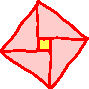
\includegraphics{logo.pdf}}

\title{杂谈勾股定理}
\subtitle{数学史讲座之一}
\institute{九章学堂}
\author{张三}
\date{\today}
\subject{勾股定理}
\keywords{勾股定理, 历史}

\begin{document}

\begin{frame}
\titlepage
\end{frame}

\begin{frame}{目录}
\tableofcontents[pausesections]
\end{frame}

\section{勾股定理在古代}
\label{sec:ancient}

\begin{frame}{古希腊数学}

勾股定理在西方称为毕达哥拉斯定理,古希腊数学家在 2000 多年前就已经发现并证明了它\cite{Kline}。\pause
\begin{itemize}
\item<+-| alert@+>
  公元前 6 世纪,毕达哥拉斯学派发现一个法则,可以构造直角三角形的边长;
\item<+-| alert@+>
  公元前 3 世纪,欧几里德《几何原本》使用面积法证明勾股定理。
\end{itemize}
\end{frame}

\begin{frame}{古中国数学}{定理发现}

中国在 3000 多年前就知道勾股数的概念,比古希腊更早一些。\pause

《周髀算经》的记载:\pause
\begin{itemize}[<+-| alert@+>]
\item
  公元前 11 世纪,商高答周公问:
\begin{quote}
勾广三,股修四,径隅五。
\end{quote}
\item
  又载公元前 7--6 世纪陈子答荣方问,表述了勾股定理的一般形式:
\begin{quote}
若求邪至日者,以日下为勾,日高为股,勾股各自乘,并而开方除之,得邪至日。
\end{quote}
\end{itemize}
\end{frame}

\begin{frame}{古中国数学}{定理证明}
有论者认为早在公元前 11 世纪商高即已证明勾股定理\cite{quanjing}。完整的证明见于三国时(公元 3 世纪)赵爽对《周髀算经》的注释。
\pause
\begin{figure}
\centering
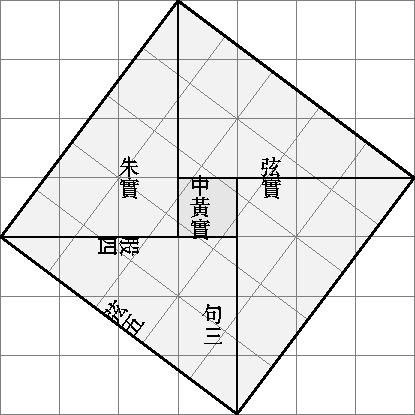
\includegraphics[height=0.4\textheight]{xiantu.pdf}
\caption{赵爽的弦图可给出勾股定理的一个富于对称美的证明}
\end{figure}
\end{frame}

\section{勾股定理在现代}

\begin{frame}{现代叙述}
\begin{thm}[勾股定理]
直角三角形斜边的平方等于两直角边的平方和。\pause

可以用符号语言表述为:设直角三角形 $ABC$,其中 $\angle C=90^\circ$,则有
\begin{equation}\label{eq:gougu}
AB^2 = BC^2 + AC^2.
\end{equation}
\begin{center}
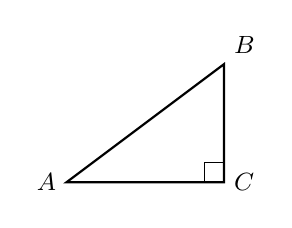
\begin{tikzpicture}[scale=0.5,font=\small]
\draw[thick] (0,0) node[left] {$A$}
   -- (4,0) node[right] {$C$}
   -- (4,3) node[above right] {$B$} -- cycle;
\draw (3.5,0) |- (4,0.5);
\end{tikzpicture}
\end{center}
\end{thm}
\end{frame}

\begin{frame}{勾股数}
满足式 \eqref{eq:gougu} 的整数称为\emph{勾股数}。第 \ref{sec:ancient} 节所说毕达哥拉斯学派得到的三元数组就是勾股数。
\begin{table}
\centering
% 颜色 craneorange 是在 crane 色彩主题中定义的
\rowcolors{2}{craneorange!25}{craneorange!50}
\begin{tabular}{rrr}
\rowcolor{craneorange}直角边 $a$ & 直角边 $b$ & 斜边 $c$\\
3 & 4 & 5 \\
5 & 12 & 13 \\
7 & 24 & 25 \\
8 & 15 & 17 \\
\end{tabular}
\caption{较小的几组勾股数}
\end{table}
\end{frame}

\begin{frame}{参考文献}
\nocite{Shiye}
\bibliography{math}
\end{frame}
\end{document}
